\section{Considerações Iniciais}

Quando se conduz uma revisão de literatura sem o pré-estabelecimento de um protocolo de revisão, há um direcionamento por interesses pessoais, o que leva a resultados pouco confiáveis. Nesse contexto, pesquisadores vêm utilizando uma técnica denominada de \sigla{MS}{Mapeamento Sistemático} para auxiliar o pesquisador a conduzir uma revisão bibliográfica de forma totalmente sistemática, com o intuito de evitar que trabalhos importantes fiquem fora de suas pesquisas. Um MS é caracterizado por ser um meio de avaliar e interpretar todas as pesquisas disponíveis, referentes a uma questão de pesquisa, tema, área ou fenômeno de interesse. O MS visa expor uma avaliação justa de um tema de pesquisa, usando uma metodologia confiável e rigorosa~\cite{Petersen_2008, Kitchenham_2010, Petersen_20151}.


De acordo com~\citeonline{Petersen_20151}, o MS é projetado para dar uma visão geral de uma área de investigação por meio da classificação e contagem de contribuições em relação a um conjunto de categorias de classificação~\cite{Petersen_2008, Kitchenham_2010}. Em outras palavras, trata-se de realizar uma vasta pesquisa na literatura, a fim de identificar quais temas já foram abordados, quais temas ainda não foram abordados e quais são novas possíveis pesquisas~\cite{Kitchenham_2010}. Existe também a técnica de \sigla{RS}{Revisão Sistemática}, a qual compartilha algumas características com o MS, como no que diz respeito à busca e seleção do estudo. Segundo~\citeonline{Petersen_20151}, tais técnicas são diferentes em termos de objetivos e, portanto, usam diferentes abordagens para a análise de dados, pois a RS visa sintetizar evidências, também considerando a força da evidência, e o MS preocupa-se principalmente com a estruturação de uma determinada área de pesquisa~\cite{Petersen_20151}. Segundo~\citeonline{Kitchenham_2010}, MS implica na forma mais adequada para se identificar, avaliar e interpretar toda uma área de pesquisa para um tema em particular. 

Resume-se, então, que um MS configura um alicerce para novas atividades de pesquisa acerca de um determinado tema. Diante disso, foi realizado um MS sobre ADM e KDM~\cite{durelli_systematic_mapping}; a motivação para realizar esse MS é identificar os temas que são mais investigados, bem como os temas que ainda não foram pesquisados no contexto da abordagem ADM e do metamodelo KDM. Embora a ADM seja uma abordagem relativamente nova, o OMG afirma que ela é uma importante abordagem, pois combina dois dos principais campos da Engenharia de Software: MDE (ver Capítulo~\ref{chapter:fundamentacao_teorica}, Seção~\ref{Cap2_Sec2_Desenvolvimento_Dirigido_a_Modelos}) e reengenharia de software. Desde a criação da ADM, muitos esforços têm enfatizado a modernização de sistemas por meio dessa abordagem. Assim, se faz necessário a condução de uma investigação mais sistemática dos temas englobados por tal área de pesquisa. Nota-se que este capítulo é uma extensão do seguinte artigo: \textit{A Mapping Study on Architecture-Driven Modernization}~\cite{durelli_systematic_mapping}.


Este capítulo está organizado da seguinte forma: Seção~\ref{sec:metodologia_pesquisa} descreve a metodologia de como o MS foi conduzido;  Subseção~\ref{subsec:estrategia_de_busca} apresenta a estratégia de busca utilizada nesse MS; a Subseção~\ref{subsec:fonte_de_estudo_e_selecao}, descreve as fontes de estudos utilizadas no MS, além disso, também apresenta como foi realizada a seleção dos estudos; a Subseção~\ref{subsec:definindo_esquema_de_classificacao} apresenta o esquema de classificação considerado no MS; na Subseção~\ref{subsec:extracao_e_sintese_do_dados}, a extração e a síntese dos dados são discutidas; na Subseção~\ref{subsec:mapeamento_e_dis}, um gráfico de bolha resultante do MS é apresentado, dando ênfase nas principais descobertas desse MS. Ainda nessa subseção, as questões de pesquisas são discutidas; a Seção~\ref{subsec:principais_constatações_e_questões_Em_Aberto} apresenta as principais constatações e questões em aberto, relacionadas à ADM e ao KDM; a Seção~\ref{subsec:ameaças_a_validade} apresenta as ameaças à validade do MS; Seção~\ref{sec:considerações_finais_do_mapeamento_sistematico} descreve as considerações finais deste capítulo.


%Seção X apresenta as principais descobertas desse MS. Na Seção X as ameaças às validades são apresentadas. Na Seção X as considerações finais são destacadas.\change{mudar e colocar a estrutura}

\section{Metodologia de Pesquisa}\label{sec:metodologia_pesquisa}

Como já salientado nas considerações iniciais, um MS fornece um processo sistemático para identificar relevantes pesquisas com o objetivo de responder específicas questões. Durante a condução desse MS, todos os passos propostos por~\citeonline{Petersen_20151, Petersen_2008} foram seguidos. Uma visão geral de todos os passos propostos por tais autores pode ser observada na Figura~\ref{fig:all_steps_MS}. Nota-se que cada passo produz um resultado intermediário e de acordo com tais autores, cinco passos são essenciais: (\textit{i}) \textit{Definition of Research Questions}, (\textit{ii}) \textit{Conducting Search}, (\textit{iii}) \emph{Screening of Papers}, (\textit{iv}) \emph{Keywording using Abstracts} e (\textit{v}) \textit{Data Extraction and Mapping Process}. 

\begin{figure}[h]
 \caption{Processo para a condução de um Mapeamento Sistemático.}
 \label{fig:all_steps_MS}
 \centering
 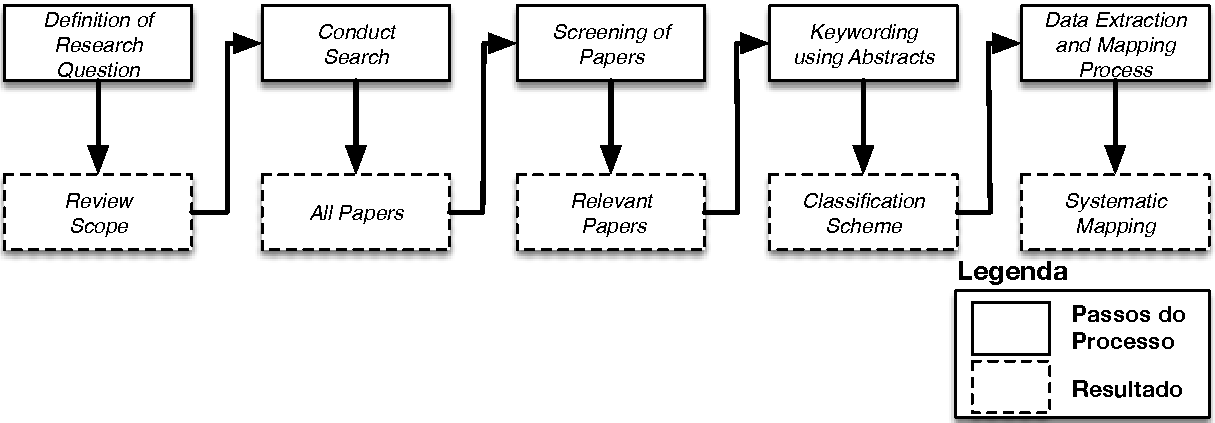
\includegraphics[scale=0.7]{images/SystematicProcessSteps_new_day_21_01}
 \fadaptada{Petersen_2008}
\end{figure}

\subsection{Estratégia de Busca}\label{subsec:estrategia_de_busca}

O protocolo do MS deve ser definido e é usualmente dividido em dois subpassos: (\textit{i}) a definição das questões de pesquisa e (\textit{ii}) a \textit{string} de busca. 

\sigla{QPs}{Questões de Pesquisas} devem englobar o propósito do MS, o qual foca a identificação e a caracterização do estado atual da ADM e do metamodelo KDM. Dessa forma, como já citado, a motivação para realizar esse MS é identificar os temas que são mais investigados, bem como os temas que ainda não foram investigados no contexto da abordagem ADM e do metamodelo KDM. A partir desses objetivos, delineiam-se as seguintes questões:

\begin{itemize}
\item \textbf{QP$_1$} - Dados os metamodelos da ADM, qual é mais utilizado na literatura? Além disso, dado o metamodelo identificado, qual (is) é (são) o (s) pacote (s) mais e menos utilizado (s)?
\item \textbf{QP$_2$} - Que tipos de estudos são publicados no contexto da ADM?
\item \textbf{QP$_3$} - Quais são as áreas mais e menos investigadas no contexto da ADM? Adicionalmente, quais são os tipos de contribuições que foram publicados até agora?
\end{itemize}

Considerando as QPs estabelecidas, definiram-se os atributos e a amplitude do MS com a técnica \sigla{PICO}{\textit{Population}, \textit{Intervention}, \textit{Comparator} e \textit{Outcomes}}~\cite{Kitchenham_2010}, e identificaram-se os termos a serem utilizados na \textit{string} de busca:

\begin{itemize}
\item Quanto à população: Em Engenharia de Software e no contexto de MS, população diz respeito à uma específica área de pesquisa. No contexto desse MS, a população são artigos publicados na literatura científica sobre algum processo, técnica ou ferramenta que utilize ADM e seus metamodelos;

\item Quanto à intervenção: Em Engenharia de Software, intervenção refere-se à metodologia de software, ferramenta, tecnologia ou procedimento. No contexto, desse MS, a intervenção são abordagens e ferramentas publicadas na literatura científica que utilizam ADM e seus metamodelos;

\item Quanto à comparação: A comparação não é aplicada no contexto desse MS;

\item Quanto aos resultados esperados: Espera-se como resultado uma visão geral dos estudos que foram publicados para a ADM e seus metamodelos, enfatizando estudos primários que descrevem técnicas, abordagens, processos e ferramentas para auxiliar o engenheiro de modernização durante a condução de modernização de sistemas legados com a utilização da abordagem ADM.

\end{itemize}

A partir dos termos identificados, define-se a \textit{string} de busca para a recuperação de estudos. Todos os termos devem ser traduzidos de acordo com o idioma dos artigos que se deseja recuperar (no contexto deste MS, inglês) e associados com sinônimos, conforme sugestões de especialistas. Na Figura~\ref{fig:string_de_busca}, é exposta a \textit{string} de busca que foi utilizada no presente MS.

\begin{figure}[h]
 \caption{\textit{String} de busca definida.}
 \label{fig:string_de_busca}
 \centering
 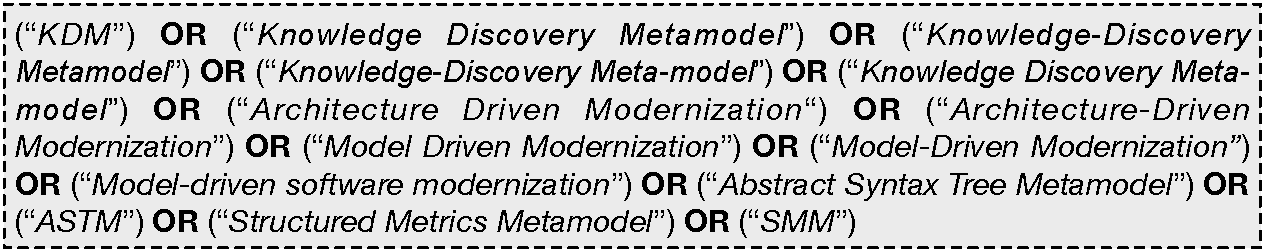
\includegraphics[scale=0.6]{images/searchStringMS}
 \fautor
\end{figure}

\subsection{Fonte de Estudos e Seleção dos Estudos}\label{subsec:fonte_de_estudo_e_selecao}

As fontes de estudos utilizadas durante o MS foram as bibliotecas digitais da \textit{ACM}, 
\textit{IEEE XPLORE}, \textit{Scopus}, \textit{Web of Science} e \textit{Engineering Village}. Tais bibliotecas digitais foram selecionadas com base na experiência reportada por~\citeonline{dyba_2015}. De acordo com esses autores, tais fontes de estudos são suficientes para identificar estudos primários relevantes. Nota-se que os recursos fornecidos por essas bibliotecas digitais, bem como a sintaxe exata da \textit{string} de busca a ser aplicada variam de uma biblioteca para outra, assim, a \textit{string} de busca apresentada na Figura~\ref{fig:string_de_busca} foi utilizada como base para construir uma \textit{string} de busca semanticamente equivalente e sob medida para cada biblioteca digital. %As \textit{strings} de buscas utilizada em todas as bibliotecas digitais pode ser visualizada na Tabela~\ref{long}.


%\begin{longtable}[!tb]{ | m{2cm} | m{12cm}| }
% \caption{Bibliotecas digitais e \textit{String} de busca adaptadas.\label{long}}\\
 
% \hline
% \multicolumn{2}{| c |}{Início da Tabela}\\
% \hline
% Bibliotecas Digitais & \textit{String} de Busca\\
% \hline
% \endfirsthead
 
% \hline
% \multicolumn{2}{|c|}{Continuação da Tabela~\ref{long}}\\
% \hline
% Bibliotecas Digitais & \textit{String} de Busca\\
% \hline
% \endhead
 
% \hline
% \endfoot
 
% \hline
% \multicolumn{2}{| c |}{Fim da Tabela}\\
% \hline\hline
% \endlastfoot
 
% ACM & ("Knowledge Discovery Metamodel" or "Knowledge-Discovery Metamodel" or "Knowledge-Discovery Meta-model" or "Knowledge Discovery Meta-model" or "Architecture Driven Modernization" or "Architecture-Driven Modernization" or "Model Driven Modernization" or "Model-Driven Modernization" or "Model-driven software modernization" or "ADM Pattern Recognition specification" or "ADM Visualization specification" or "ADM Refactoring specification" or "ADM Transformation specification" or "KDM Metamodel" or "KDM Meta-model" or "Software Metrics Meta-model" or "Software Metrics Metamodel" or "Structured Metrics Meta-Model" or "Structured Metrics Metamodel" or "Abstract Syntax Tree Metamodel" or "Abstract Syntax Tree Meta-model")\\
 %\hline
 %IEEE XPLORE & ((((((((((((((((((((("Knowledge Discovery Metamodel") OR "Knowledge-Discovery Metamodel") OR "Knowledge-Discovery Meta-model") OR "Knowledge Discovery Meta-model") OR "Architecture Driven Modernization") OR "Architecture-Driven Modernization") OR "Model Driven Modernization") OR "Model-Driven Modernization") OR "Model-driven software modernization") OR "ADM Pattern Recognition specification") OR "ADM Visualization specification") OR "ADM Refactoring specification") OR "ADM Transformation specification") OR "KDM Metamodel") OR "KDM Meta-model") OR "Software Metrics Meta-model") OR "Software Metrics Metamodel") OR "Structured Metrics Meta-Model") OR "Structured Metrics Metamodel") OR "Abstract Syntax Tree Metamodel") OR "Abstract Syntax Tree Meta-model")\\
 %\hline
 %Scopus & ("Knowledge Discovery Metamodel"  OR  "Knowledge-Discovery Metamodel"  OR  "Knowledge-Discovery Meta-model"  OR  "Knowledge Discovery Meta-model"  OR  "Architecture Driven Modernization" OR  "Architecture-Driven Modernization"  OR  "Model Driven Modernization"  OR  "Model-Driven Modernization"  OR  "Model-driven software modernization"  OR  "ADM Pattern Recognition specification"  OR  "ADM Visualization specification"  OR  "ADM Refactoring specification"  OR  "ADM Transformation specification"  OR  "KDM Metamodel"  OR  "KDM Meta-model"  OR  "Software Metrics Meta-model"  OR  "Software Metrics Metamodel"  OR  "Structured Metrics Meta-Model"  OR  "Structured Metrics Metamodel"  OR  "Abstract Syntax Tree Metamodel"  OR  "Abstract Syntax Tree Meta-model")\\
 %\hline
 %Web of Science & ("Knowledge Discovery Metamodel" OR "Knowledge-Discovery Metamodel" OR "Knowledge-Discovery Meta-model" OR "Knowledge Discovery Meta-model" OR "Architecture Driven Modernization" OR "Architecture-Driven Modernization" OR "Model Driven Modernization" OR "Model-Driven Modernization" OR "Model-driven software modernization" OR "ADM Pattern Recognition specification" OR "ADM Visualization specification" OR "ADM Refactoring specification" OR "ADM Transformation specification" OR "KDM Metamodel" OR "KDM Meta-model" OR "Software Metrics Meta-model" OR "Software Metrics Metamodel" OR "Structured Metrics Meta-Model" OR "Structured Metrics Metamodel" OR "Abstract Syntax Tree Metamodel" OR "Abstract Syntax Tree Meta-model")\\
 %\hline
 %Engeneering Village & "Knowledge Discovery Metamodel" OR "Knowledge-Discovery Metamodel" OR "Knowledge-Discovery Meta-model" OR "Knowledge Discovery Meta-model" OR "Architecture Driven Modernization" OR "Architecture-Driven Modernization" OR "Model Driven Modernization" OR "Model-Driven Modernization" OR "Model-driven software modernization" OR "ADM Pattern Recognition specification" OR "ADM Visualization specification" OR "ADM Refactoring specification" OR "ADM Transformation specification" OR "KDM Metamodel" OR "KDM Meta-model" OR "Software Metrics Meta-model" OR "Software Metrics Metamodel" OR "Structured Metrics Meta-Model" OR "Structured Metrics Metamodel" OR "Abstract Syntax Tree Metamodel" OR "Abstract Syntax Tree Meta-model"\\
 %\hline
 %Google Scholar & ("Knowledge Discovery Metamodel" or "Knowledge-Discovery Metamodel" or "Knowledge-Discovery Meta-model" or "Knowledge Discovery Meta-model" or "Architecture Driven Modernization" or "Architecture-Driven Modernization" or "Model Driven Modernization" or "Model-Driven Modernization" or "Model-driven software modernization" or "ADM Pattern Recognition specification" or "ADM Visualization specification" or "ADM Refactoring specification" or "ADM Transformation specification" or "KDM Metamodel" or "KDM Meta-model" or "Software Metrics Meta-model" or "Software Metrics Metamodel" or "Structured Metrics Meta-Model" or "Structured Metrics Metamodel" or "Abstract Syntax Tree Metamodel" or "Abstract Syntax Tree Meta-model")\\
 %\hline
 %\end{longtable}

Para determinar quais estudos primários são relevantes para responder às QPs, definiu-se um conjunto de critérios de inclusão.

\begin{itemize}
\item Critérios de Inclusão:
    \begin{itemize}
    \item O estudo primário apresenta pelo menos uma abordagem de modernização que utiliza ADM e seus metamodelos;
    \item O estudo primário descreve uma avaliação empírica da abordagem que utiliza ADM.
    \end{itemize}
\end{itemize}

Similarmente, também foram definidos três critérios de exclusão, a saber:

\begin{itemize}
\item Critérios de Exclusão:
    \begin{itemize}
    \item Artigos que mencionam a ADM e seus metamodelos apenas no \textit{abstract};
    \item Artigos introdutórios para livros e \textit{workshops};
    \item O estudo primário é um artigo pequeno (\textit{short paper}), o qual contém até três páginas.
    \end{itemize}
\end{itemize}

A Scopus foi a biblioteca digital que retornou mais estudos primários, 58\% (150) (ver Figura~\ref{fig:distribuicao_biblioteca_digital}). Por outro lado, foram recuperados 20\% (51) estudos da ACM, 12\% (30) da Engineering Village, 6\% (17) da Web of Science e 4\% (11) da IEEE. 

\begin{figure}[h]
 \caption{Distribuição dos estudos primários de cada biblioteca digital.}
 \label{fig:distribuicao_biblioteca_digital}
 \centering
 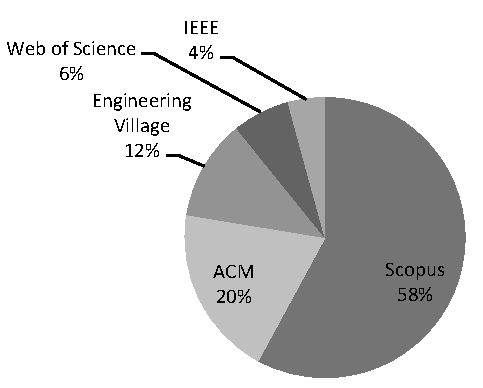
\includegraphics[scale=0.9]{images/retornoDasBasesMS}
 \fautor
\end{figure}

Somando todas as bibliotecas digitais, obtiveram-se 259 estudos primários no primeiro passo, como ilustrado na Figura~\ref{fig:todos_os_passos}. Após o primeiro passo (ver Figura~\ref{fig:todos_os_passos}), 82 artigos foram selecionados, sendo possível notar que apenas publicações de conferências e \textit{journals} foram considerados nesse MS. Posteriormente, os critérios de inclusão anteriormente apresentados foram aplicados para os 82 artigos selecionados. Após esse passo, 30 estudos primários foram considerados para serem analisados no MS como mostrado na Figura~\ref{fig:todos_os_passos}.

\begin{figure}[h]
 \caption{Todos os passos conduzidos no MS.}
 \label{fig:todos_os_passos}
 \centering
 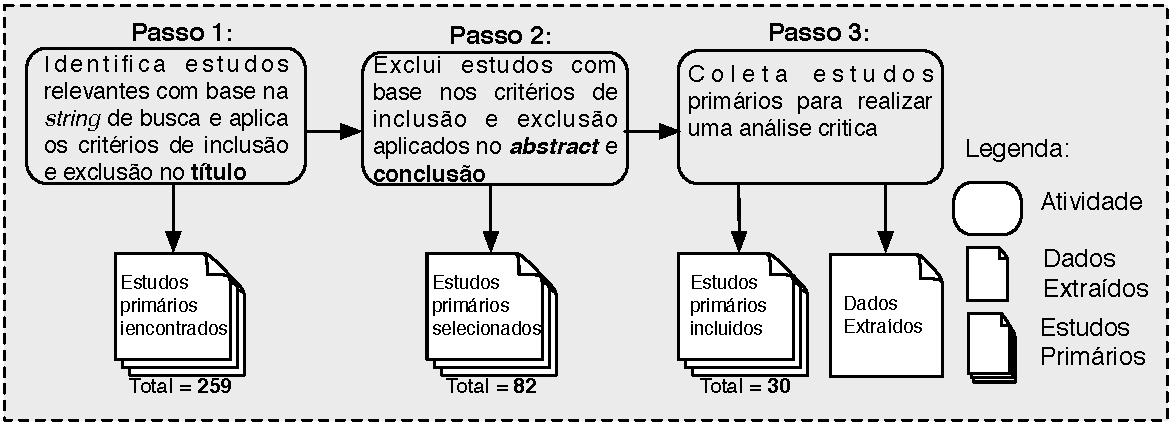
\includegraphics[scale=0.7]{images/todosOsPassosMS}
 \fautor
\end{figure}

\subsection{Definindo um Esquema de Classificação}\label{subsec:definindo_esquema_de_classificacao}

O esquema de classificação utilizado no MS foi o esquema proposto por~\citeonline{Petersen_2008, Petersen_20151} que classifica cada publicação entre categorias de acordo com três perspectivas: (\textit{i}) \textbf{Área de Foco}, (\textit{ii}) \textbf{Tipo de Contribuição} e (\textit{iii}) \textbf{Tipo de Pesquisa}. O esquema de classificação resultante é descrito a seguir.

\begin{itemize}
\item \textbf{Área de Foco}: Após ler os estudos primários, foram identificadas cinco principais áreas de foco: 
    
    \begin{itemize}
        \item \aspas{\textbf{Modernização de Software}}: está relacionada com estudos primários que descrevem abordagens que empregam ADM para modernizar sistemas legados para outra plataforma ou arquitetura;
        \item \aspas{\textbf{Extração de \textit{Business Knowledge}}}: descreve estudos primários que apresentam processos, métodos ou abordagens para extrair informações de negócio de sistemas legados;
        \item \aspas{\textbf{Extração de Interesse}}: representa estudos primários que descrevem processos, métodos ou abordagens para extrair interesses transversais de sistemas legados;
        \item \aspas{\textbf{Extensão dos metamodelos da ADM}}: descreve estudos primários que apresentam abordagens, métodos ou processos para estender um determinado metamodelo da ADM;
        \item \aspas{\textbf{Aplicabilidade}}: inclui estudos primários que buscam representar a evidência da utilização da ADM e seus metamodelos na prática, ou seja, artigos que apresentam pesquisas ou relatórios para facilitar o entendimento da ADM e seus metamodelos.
    \end{itemize}
    
    \item \textbf{Tipo de Contribuição}: Similarmente, também foram identificados cinco tipos de contribuições:
        
        \begin{itemize}
            \item \aspas{\textbf{Ferramentas}}: estudos primários que apresentam ferramentas para auxiliar a modernização de sistemas legados utilizando ADM e seus metamodelos;
            \item \aspas{\textbf{Processo}}: estudos primários que descrevem processos para auxiliar a modernização de sistemas legados utilizando ADM e seus metamodelos;
            \item \aspas{\textbf{Transformação de Modelos}}: estudos primários que descrevem o uso de linguagens de transformações para realizar transformações entre os metamodelos da ADM;
            \item \aspas{\textbf{Metamodelos}}: estudos primários que relatam extensão nos metamodelos da ADM para suprir um específico problema, por exemplo, fornecer uma extensão leve para o metamodelo KDM representar o paradigma orientado a aspecto;
            \item \aspas{\textbf{Métricas}}: estudos primários que se concentram em propor ou aplicar métricas para medir a eficácia de ADM e seus metamodelos.
        \end{itemize}
        
        \item \textbf{Tipo de Pesquisa}: reflete a abordagem de pesquisa que foi utilizada no estudo primário, e essa categoria foi criada com base no esquema proposto por~\citeonline{Wieringa_2005}:
        
        \begin{itemize}
            \item \aspas{\textbf{Pesquisa de validação}}: tem por objetivo analisar uma proposta de solução que ainda não foi aplicada na prática. A validação é realizada de uma forma sistemática e pode apresentar qualquer um destes tipos: protótipos, análise matemática, etc.;
            \item \aspas{\textbf{Pesquisa de avaliação}}: em contraste com a pesquisa de validação, pesquisa de avaliação visa examinar uma solução que já foi praticamente aplicada. Estudos nessa categoria investigam a aplicação na prática da solução proposta e, geralmente, os resultados obtidos utilizando estratégias empíricas (por exemplo, experimentos e estudo de casos);
            \item \aspas{\textbf{Proposta conceitual}}: apresenta um arranjo de coisas que já existem, de uma nova maneira. No entanto, isso não resolve precisamente um problema particular. Podem ser incluídos taxonomias, referenciais teóricos, etc.;
            \item \aspas{\textbf{Artigo descrevendo experiência}}: artigos que descrevem sobre a experiência pessoal do autor para um ou mais projetos. O autor geralmente apresenta como o projeto foi feito e o que foi realizado;
            \item \aspas{\textbf{Artigo descrevendo opinião}}: artigos que descrevem a opinião pessoal do autor sobre a adequação ou inadequação de uma técnica ou ferramenta específica.
        \end{itemize}
    
\end{itemize}


\subsection{Extração e Síntese dos Dados}\label{subsec:extracao_e_sintese_do_dados}

Os 30 estudos selecionados na etapa anterior foram analisados. Criou-se, então, um formulário para auxiliar a extração de dados, abordando os seguintes aspectos: (\textit{i}) dados relevantes sobre como a ADM e seus metamodelos são utilizados na literatura, (\textit{ii}) a data de quando a extração do dado foi realizada, (\textit{iii}) o título do estudo primário, (\textit{iv}) os autores do estudo primário, (\textit{v}) o veículo de publicação e (\textit{vi}) um resumo destacando as principais contribuições do estudo primário para posteriormente realizar a classificação. Durante o processo de extração, informações sobre cada estudo primário foram independentemente coletadas por todos os pesquisados que participaram do MS. É importante destacar que a primeira execução desse MS foi realizada em novembro de 2013, posteriormente, foi conduzido novamente em agosto de 2015 com o objetivo de atualizá-lo.

\subsection{Mapeamento e discussão das QPs}\label{subsec:mapeamento_e_dis}

O foco desta seção é apresentar uma visão geral de como a ADM e seus metamodelos são pesquisados e utilizados na literatura, bem como identificar possíveis grupos de evidências (ou seja, onde pode haver margem para uma literatura mais completa) e deserto de evidências (ou seja, onde melhores ou novas pesquisas são necessárias) de pesquisas. Além de apresentar essa visão geral, a presente seção almeja destacar respostas para as QPs definidas anteriormente.

Em vez de utilizar tabelas de frequência, foi produzido um gráfico de bolha para reportar a frequência e distribuição dos estudos primários selecionados de acordo com suas categorias e data de publicação. Argumenta-se que esse gráfico de bolha representa um mapa geral de como a ADM e seus metamodelos são utilizados na literatura. O mapa resultante é apresentado na Figura~\ref{fig:mapa_mapeamento_sistematico}.


\begin{figure}[h]
 \caption{Visão geral da pesquisa sobre ADM e seus metamodelos.}
 \label{fig:mapa_mapeamento_sistematico}
 \centering
 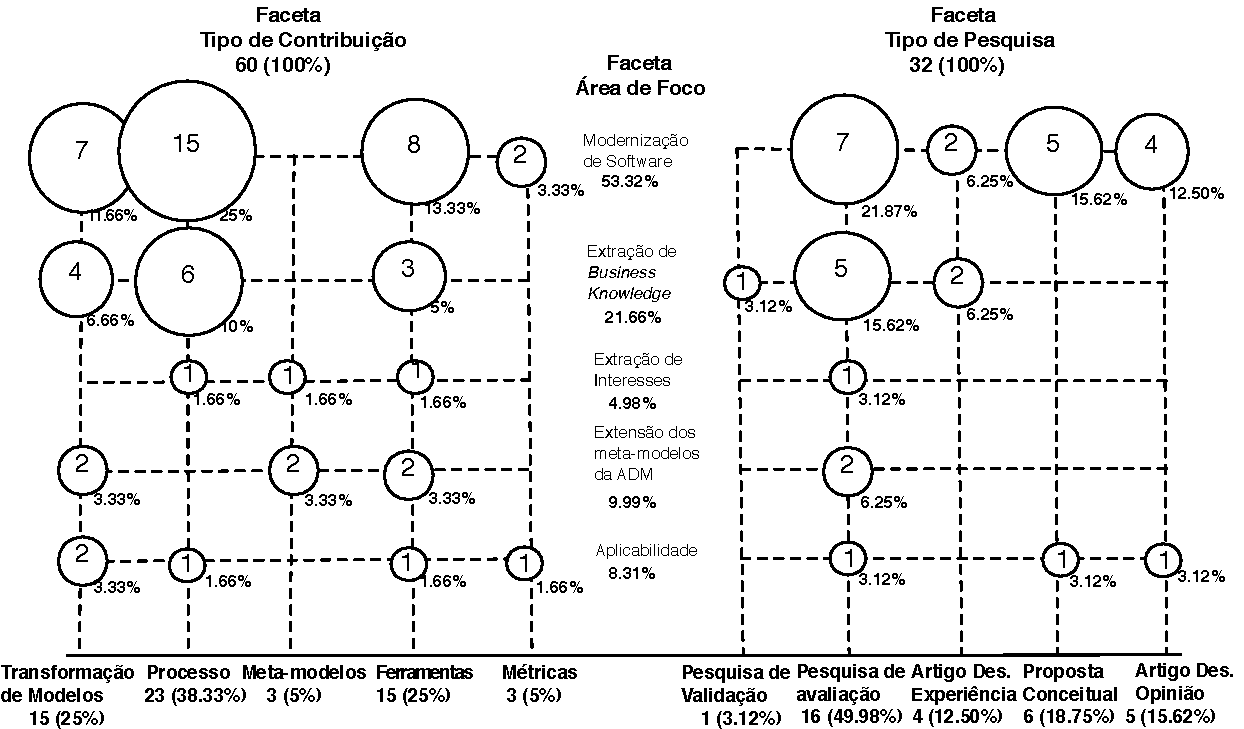
\includegraphics[scale=0.8]{images/MapaMS_port}
 \fautor
\end{figure}

Como pode ser observado, esse gráfico de bolha contém dois vértices, X e Y, os quais possuem bolhas em cada categoria. É visto que o tamanho de cada bolha representa o número de estudos primários que foram classificados em uma categoria específica. Esse gráfico é um resumo visual e fornece uma visão panorâmica que permite identificar quais são as categorias que foram salientadas em pesquisas anteriores, além disso, é possível identificar facilmente lacunas e oportunidades para futuras pesquisas. O gráfico de bolha apresentado na Figura~\ref{fig:mapa_mapeamento_sistematico} contém três facetas: \textbf{Tipo de Contribuição}, \textbf{Área de Foco} e \textbf{Tipo de Pesquisa}. Embora 30 estudos primários foram considerados no presente MS, é importante mencionar que para o gráfico de bolha alguns estudos primários foram agrupados em mais de uma categoria. Por exemplo, para o gráfico de bolha apresentado na Figura~\ref{fig:mapa_mapeamento_sistematico}, a soma dos estudos primários agrupados em cada faceta é maior do que o número de estudos primários selecionados, e isso acontece uma vez que um determinado estudo primário pode ser classificado em diversas facetas e categorias.

Para responder a primeira parte da \textbf{QP$_1$}, foram analisados todos os estudos primários, concentrando-se na identificação de qual metamodelo da ADM tem sido mais utilizado na literatura. Na Figura~\ref{fig:frequencia_kdm_packages}, lado esquerdo, são exibidos os metamodelos da ADM utilizados na literatura. Como pode ser observado, o metamodelo KDM é o mais utilizado, tendo uma frequência de 66.67\%. Em seguida, o segundo metamodelo mais utilizado é o SMM - 10\% dos estudos primários relatam a utilização desse metamodelo. O metamodelo ASTM foi utilizado em apenas 6.66\% dos estudos primários. 16.66\% dos estudos primários não mencionam explicitamente qual metamodelo foi utilizado durante o processo de modernização conduzido, apenas citam e relatam a utilização da ADM.

\begin{figure}[!h]
\caption{Frequência de utilização dos metamodelos da ADM e frequência de utilização dos seus pacotes.}
 \label{fig:frequencia_kdm_packages}
\centering
\begin{minipage}{.5\textwidth}
  \centering
  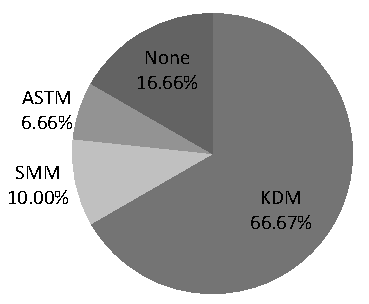
\includegraphics[scale=0.9]{images/MetamodelosDIstribuition}
\end{minipage}%
\begin{minipage}{.5\textwidth}
  \centering
  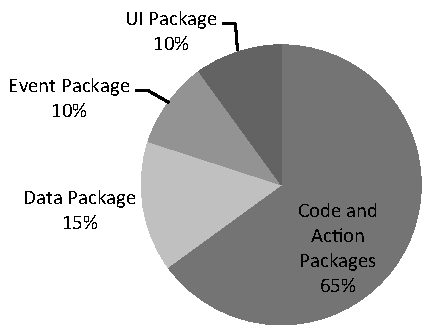
\includegraphics[scale=0.9]{images/PacotesKDM}
\end{minipage}
\fautor
\end{figure}

Para responder a segunda parte da \textbf{QP$_1$}, foram analisados quais pacotes são mais e menos utilizados dentro do metamodelo KDM. Na Figura~\ref{fig:frequencia_kdm_packages}, lado direito, é evidente que os pacotes \texttt{Code} e \texttt{Action} são os mais utilizados na literatura, contendo uma frequência de 65\%. Acredita-se que a razão para essa frequência tão alta seja por dois principais motivos: (\textit{i}) tais pacotes representam o código-fonte de um determinado sistema, além disso, a maioria das abordagens identificadas utiliza como entrada o código-fonte de sistemas que almejam modernizar seguindo a ADM e seus metamodelos; (\textit{ii}) outros pacotes do KDM ainda não possuem ferramentas para realizar a instanciação de forma automática, ou seja, existe uma limitação de \textit{parsers} que análisa outros tipos de artefatos de um determinado sistema para criar uma representação mais fiel do sistema, não apenas do código-fonte. O terceiro pacote mais utilizado é o \texttt{Data}, o qual é utilizado para representar dados,  tais como banco de dados, registros, etc. Os pacotes \texttt{Event} e \texttt{UI} foram utilizados 10\%. Outros pacotes do metamodelo KDM não foram explicitamente mencionados nos estudos primários identificados.

Observando a faceta \textbf{Tipo de Pesquisa}, lado direito da Figura~\ref{fig:mapa_mapeamento_sistematico}, é possível responder a \textbf{QP$_2$}. A maioria dos estudos primários identificados foi classificado como \aspas{\textbf{Pesquisa de Avaliação}}, aproximadamente 49\%. Uma pequena porcentagem de estudos primários foi classificada como \aspas{\textbf{Pesquisa de Validação}} - apenas 3.12\%. 12.50\% dos estudos primários identificados descrevem a experiência dos autores (\aspas{\textbf{Artigo Des. Experiência}}) com a utilização da ADM e de seus metamodelos. 18.75\% foram agrupas em \aspas{\textbf{Proposta Conceitual}} e \aspas{\textbf{Artigos Des. Opinião}} teve a frequência de 15.62\%.

Ainda em relação à Figura~\ref{fig:mapa_mapeamento_sistematico} na faceta \textbf{Tipo de Contribuição}, lado esquerdo, é visto que a maioria dos estudos primários identificados apresenta \aspas{\textbf{processos}} para auxiliar os engenheiros de software durante a modernização de sistemas legados. Também foi identificado um total de 15 estudos primários (25\%) que apresentam algum tipo de \aspas{\textbf{transformação de modelos}} utilizando os metamodelos da ADM. Similarmente, 15 estudos primários (25\%) demonstram ferramentas para auxiliar o engenheiro de software durante a condução da modernização utilizando ADM e seus metamodelos. Acredita-se que esses dois últimos resultados foram obtidos uma vez que a maioria dos estudos primários identificados descreve processos de modernização, assim, pesquisadores devem criar um conjunto de transformações de modelos e ferramentas para automatizar parcialmente ou totalmente o processo proposto.

Por outro lado, \aspas{\textbf{metamodelos}} e \aspas{\textbf{métricas}} são as contribuições com menos estudos primários identificados, 5\% cada. Com isso, argumenta-se que os estudos primários que descrevem \aspas{\textbf{processos}} para ajudar a modernização dos sistemas legados por meio da ADM, os estudos que apresentam \aspas{\textbf{transformação de modelos}} entre os metamodelos da ADM (KDM, SMM e ASTM) e os artigos que descrevem ferramentas para automatizar parcialmente ou totalmente o processo da ADM podem ser considerados como grupos de evidências. E os \aspas{\textbf{metamodelos}} (artigos que explicam e/ou apresentam como estender metamodelos da ADM) e \aspas{\textbf{métricas}} (artigos que descrevem como aplicar métricas nos metamodelos da ADM) podem ser considerados como deserto de evidência, evidenciando que novos estudos primários são necessários.

Considerando o centro da Figura~\ref{fig:mapa_mapeamento_sistematico}, faceta \textbf{Área de Foco}, é possível visualizar que a maioria dos estudos primários identificados foi classificado como \aspas{\textbf{Modernização de Software}}, um total de 53.32\%. Em seguida, 21.66\% dos estudos primários foram categorizados em \aspas{\textbf{Extração de \textit{Business Knowledge}}}. \aspas{\textbf{Extração de Interesses}}, \aspas{\textbf{Extensão dos metamodelos da ADM}} e \aspas{\textbf{Aplicabilidade}}, coletivamente, representam uma porcentagem de aproximadamente 25\% dos estudos primários. Como resultado dessa análise, foi possível responder parcialmente a \textbf{QP$_3$}, ou seja, os principais \textbf{Tipo de Contribuição} relacionado à ADM e seus metamodelos disponíveis na literatura e identificados no MS foram destacados. A resposta conclusiva e completa da \textbf{QP$_3$} é apresentada a seguir. Para facilitar o entendimento e a organização deste mapeamento cada \textbf{Área de Foco} identificado no MS é apresentado em uma subseção.


\subsubsection{Modernização de Software} % (fold)
\label{ssub:approach}

\citeonline{6311013} propõem \textbf{GAFEMO}, a qual é uma abordagem para auxiliar a modernização de sistemas legados em sistemas orientados a serviço. Essa abordagem utiliza como entrada o sistema legado e, então, cria uma instância do metamodelo KDM para representar o código-fonte do sistema legado. Posteriormente, os autores definiram um conjunto de transformações para serem aplicadas nessa instância do KDM almejando criar os serviços.


 %Jorge Maratalla et al., propose \textbf{GAFEMO}~\cite{6311013}, which aims to modernize a legacy systems to the service-oriented approach taking advantage of the features provided by gap-analysis techniques. This approach takes as input a legacy system and then creates KDM representations of it. Afterwards, a set of rules are applied in this model to create the services.

%In~\cite{Mazon:2007:MDM:1784489.1784497} the authors propose a modernization approach for the modernization of Data warehouses following the concepts of ADM. The approach automatically performs the following tasks: (\textit{i}) obtain a logical representation of data sources (\textit{ii}) mark this logical representation with MD concepts, and (\textit{iii}) derive a conceptual MD model from the marked model.

%\citeonline{Mazon:2007:MDM:1784489.1784497} apresentam uma abordagem para modernizar

\citeonline{Mazon:2007:MDM:1784489.1784497} definiram uma abordagem para modernizar \textit{data warehouses} seguindo os conceitos da ADM. Essa abordagem automaticamente executa as seguintes tarefas: (\textit{i}) obtém uma representação lógica das fontes de dados; (\textit{ii}) posteriormente, essa representação lógica é anotada e transformada em instância do KDM; (\textit{iii}) em seguida, a instância do KDM é transformada em um modelo de análise de dados multidimensional. Similarmente, \citeonline{Guzman:2007:AAR:1339262.1339532} definem uma abordagem para realizar a análise de sistemas legados e criar funcionalidades para serem expostas como serviços, usando conceitos de \textit{Web Services} juntamente com a ADM.



%In~\cite{Guzman:2007:AAR:1339262.1339532} is defined an approach that is focused on the analysis of legacy systems to discover and create functionalities to be exposed as services using Web Services by means of ADM. 
%It is based in five steps: (\textit{i}) Database reverse engineering: database schema is reversed and a suitable model is built; (\textit{ii}) First service extraction: based on the structure of the database schema, a first service extraction can be undertaken; (\textit{iii}) PIM generation: is obtained from the PSM representation using a model-to-model transformation, CRUD operations are automatically created; (\textit{iv}) Service discovering: abstract objects are identified in the PIM; (\textit{v}) WSDL (Web Service Description Language) generation: using the PIM, a model-to-model transformation and a WSDL  metamodel are generated to expose the services discovered and created in the PIM and the PSM. 

Em~\citeonline{5741334, SMR:SMR582} os autores desenvolveram uma abordagem seguindo as diretrizes da ADM denominada \aspas{CloudMIG}. Essa abordagem pretende fornecer software como serviço (do inglês - \sigla{SaaS}{\textit{Software as a Service}}). %Essa abordagem consiste de seis principais passos: (\textit{i}) extração: inclui a extração da arquitetura e instanciação do sistema em nível do metamodelo KDM, (\textit{ii}) seleção: 
Do mesmo modo, \citeonline{4400179} também desenvolveu uma abordagem para utilizar ADM e seus metamodelos, principalmente o KDM, para analisar sistemas legados, descobrir e criar funcionalidades para serem expostas como serviços, utilizando os conceitos de \textit{Web Services}.

%In~\cite{5741334, SMR:SMR582} is proposed an approach based on ADM named CloudMIG that aims at supporting SaaS (Software as a Service) providers to semi-automatically migrate legacy software systems to the cloud. It is composed of six major steps: (\textit{i}) Extraction: Includes the extraction of architectural and utilization models of the legacy system, the approach uses KDM; (\textit{ii}) Selection: Select an appropriate CEM- compatible cloud profile candidate; (\textit{iii}) Generation: Produces the target architecture and a mapping model; (\textit{iv}) Adaptation: The adaptation activity enables a reengineer to manually adjust the target architecture; (\textit{v}) Evaluation: Realize static analyses and a runtime simulation of the target architecture; (\textit{vi}) Transformation: The actual transformation of the existing system from the generated target architecture to the aimed cloud environment. In~\cite{4400179} the authors propose an approach that uses ADM which is focused on the analysis of legacy systems to discover and create functionalities to be exposed as services using Web Services.

\citeonline{5328801, delCastillo:2009:PRP:1529282.1529753, ICEISPerez:CastilloGCP12} apresentam uma abordagem para modernizar sistemas legados juntamente com o banco de dados relacional. Mais especificamente, essa abordagem obtém três principais modelos seguindo a abordagem ADM. Primeiro, tal abordagem recupera uma instância do pacote \texttt{Code} do metamodelo KDM. Em seguida, uma instância do pacote \texttt{Data} do metamodelo KDM também é recuperada para representar o banco de dados relacional. Essa segunda instância é recuperada com base nas \textit{embedded SQL}, que são encontradas no código-fonte. O objetivo é separar tais SQL para facilitar a modularidade e futuras manutenções. Depois, transformações de modelos são executadas e o sistema legado é modernizado.

 %P\'{e}rez-Castillo et al.,~\cite{5328801, delCastillo:2009:PRP:1529282.1529753, ICEISPerez:CastilloGCP12} present  approaches to modernize legacy systems together with the legacy relational database. This approach recovers the code-to-data linkages and obtains three kinds of models according to the ADM approach: (\textit{i}) The KDM Code Model, which represents the inventory of legacy source code. It has also the points that link the SQL Sentence Models and Database Schema Models. (\textit{ii}) The SQL Sentence Model for modeling a certain SQL query that was embedded in legacy source code. (\textit{iii}) The Database Schema Model, which represents the specific database fragment derived by an SQL Sentence Model. 


~\citeonline{FuentesFernandez2012247} apresentam uma abordagem de modernização denominada XIRUP, interativa e estruturada em quatro fases: (\textit{i}) avaliação preliminar,
(\textit{ii}) compreensão, (\textit{iii}) construção e (\textit{iv}) migração. Essa abordagem de modernização é baseada em componentes, com foco no levantamento inicial de informações-chave, e depende de uma abordagem orientada a modelos, com o uso extensivo da experiência dos projetos anteriores. 

~\citeonline{Mainetti:2012:MMT:2364120.2364182} apresentam uma abordagem que permite desenvolvedores automaticamente modernizar a interface gráfica de um determinado sistema legado para \sigla{RIA}{\textit{Rich Internet Application}}.
%
%
%Mainetti et al.,~\cite{Mainetti:2012:MMT:2364120.2364182} present an approach that allows developers to automatically modernize the client side of legacy systems. In this approach developers can refactor the Graphical User Interface (GUI) of legacy systems during the modernization, taking the opportunities offered by novel interaction paradigms, i.e.,  
%
 Similarmente, \citeonline{Rodriguez-Echeverria:2011:MLW:2186508.2186536} também apresentam uma abordagem de modernização que utiliza os metamodelos da ADM para definir um processo sistemático com o objetivo de transformar aplicações web em RIA.
 
 %In~\cite{Rodriguez-Echeverria:2011:MLW:2186508.2186536} the authors present an approach for the definition of a systematic process for Web Applications (WA) to RIA modernization, by applying ADM principles. The approach presented by the authors consists on generating a RIA client from the legacy WA presentation and navigation layers and its corresponding service-oriented connection layer with the underlying business logic at server side. 
 
 
 
 
~\citeonline{6385130} definem uma abordagem que ajuda na construção de distintas visões arquiteturais de sistemas legados. Assim, os autores criaram um conjunto de algoritmos de agrupamento que é conduzido por meio de visões arquiteturais comuns. Essa abordagem faz
utilização do metamodelo KDM. ~\citeonline{5440163} utilizam os conceitos da ADM para construir uma ferramenta de modernização, visando gerar relatórios de métricas para avaliar os esforços de migração. Os autores desenvolveram um extrator que gera instâncias do metamodelo KDM a partir de código PS-SQL, ou seja, transformaram PS-SQL para instâncias do metamodelo KDM, e, em seguida, relatórios de métricas foram gerados para o metamodelo KDM.

 
 %Boussaidi et al.,~\cite{6385130} propose an approach that makes use of the KDM to reconstruct and document software architectural views of the legacy system. They consider an architectural view to be a way of partitioning a system using a specific set of KDM relevant concepts and relations and they propose clustering algorithms that target specific views mainly a layered view that we call horizontal view and a feature based view that we call vertical view. In~\cite{5440163} ADM is used into practice by building a modernization tool to generate metric reports of legacy Oracle Forms applications to assess migration efforts. The authors devised an extractor that generates KDM models from PL-SQL code (PL/SQL-to-KDM) and a metrics report generator for these KDM models. 

\subsubsection{Extração de \textit{Business Knowledge}}
\label{ssub:Business_Knowledge_Extraction}

~\citeonline{Perez-Castillo:2011:ECS:1982185.1982249,6080834, 6498507,Perez-Castillo:2010:IBP:1875847.1875861} apresentam uma abordagem para recuperar regras de negócio de um determinado sistema legado, com base na ADM e no KDM. Essa abordagem é baseada em um conjunto de transformações: (\textit{i}) vários PSM são recuperados de acordo com específicos artefatos do sistema legado, (\textit{ii}) posteriormente, tais PSM são transformados em uma instância do metamodelo KDM, (\textit{iii}) em seguida, o metamodelo KDM é transformado em um modelo específico para definir regras de negócio. Além disso, os autores realizaram um conjunto de estudo de caso para verificar a eficiência e a eficácia da abordagem~\cite{PerezCastillo20121370}.

~\citeonline{Perez-Castillo:2012:IEL:2231936.2231949} também fornecem uma técnica semiautomática baseada em análise dinâmica, combinada com análise estática para instrumentar o código-fonte, com o objetivo de descobrir e obter processos de negócios em nível do metamodelo KDM. ~\citeonline{Perez-Castillo:2010:IBP:1875847.1875861} apresentam e descrevem com detalhes todas as transformações entre o metamodelo KDM e o metamodelo \sigla{BPMN}{\textit{Business Process Model and Notation}}. 

~\citeonline{lastDAyOFMyLife} apresentam uma abordagem que facilita a compreensão de um determinado software, permitindo a rastreabilidade de regras de negócios e cenários de negócios no sistema de software. A abordagem visa extrair conhecimentos específicos de negócios a partir do conhecimento sobre o sistema de software existente, representados no KDM. ~\citeonline{Fernandez-Ropero:2012:EAB:2367051.2367064} descrevem um conjunto de regras para transformar o metamodelo \textit{Mining} XML, o qual é utilizado para representar a sequência de atividades de negócios executados para o metamodelo KDM. 






%apresentam uma abordagem que facilita 
%Normantas and Vasilecas~\cite{lastDAyOFMyLife} present an approach that facilitates software comprehension by enabling traceability of business rules and business scenarios in software system, i.e., their approach aim to extract business specific knowledge from the knowledge about the existing software system represented within the KDM. Ropero et al.,~\cite{Fernandez-Ropero:2012:EAB:2367051.2367064} describes a set of rules to transform Mining XML (MXML) metamodel, which is common used to represent the sequence of business activities executed by an enterprise system to KDM. The authors takes an MXML model and obtains an equivalent KDM model at the same abstraction level. The proposed set of rules consist of eight declarative transformation rules. 

\subsubsection{Extração de Interesses} % (fold)
\label{ssub:Concern Extracting}

\citeonline{dani_san, dani_san_tool, daniel_san_journal} definem uma abordagem denominada CCKDM para auxiliar a identificação de interesses transversais utilizando uma combinação de bibliotecas de interesses com o algoritmo de mineração de dados K-means. A abordagem possui quatro passos  e dois deles são opcionais. A entrada ao processo é uma instância do metamodelo KDM e as saídas são a mesma instância do KDM com anotações dos interesses transversais identificados e alguns arquivos de registros (\textit{logs}). A identificação é realizada por meio de uma biblioteca de interesses em conjunto com o repositório de elementos KDM. A abordagem é explicada de forma que possa ser replicada por outros pesquisadores que tenham interesse em modificá-la e/ou estendê-la.

\subsubsection{Extensão dos metamodelos da ADM} % (fold)
\label{ssub:extension_of_adm_s_metamodels}

~\citeonline{5773392} definem uma extensão do metamodelo KDM denominada \sigla{COMO}{\textit{Component-Oriented MOdernization}}. De acordo com os autores, KDM suporta apenas parcialmente os conceitos de componentes. Dessa forma, a extensão COMO objetiva suprir tal limitação do metamodelo KDM. Assim, novas metaclasses são definidas para detalhar conceitos específicos relacionados com componentes. Similarmente, ~\citeonline{Perez-Castillo:2012:IEL:2231936.2231949} definem uma extensão para o metamodelo KDM que visa melhorar a representação de arquivos de registros (\textit{logs}). Porém, diferentemente da abordagem COMO, os autores não criam novas metaclasses para o metamodelo KDM, apenas utilizam anotações. ~\citeonline{library7329} define uma extensão para o metamodelo KDM para representar todos os elementos do paradigma de programação orientada a aspectos, ou seja, novas metaclasses como \texttt{Aspect}, \texttt{Advice} e \texttt{Point-cut} podem ser instanciadas para representar conceitos do paradigma de programação orientada a aspecto por meio desse KDM estendido.


\subsubsection{Aplicabilidade} % (fold)
\label{ssub:applicability}

%We also identified a small number of papers that address just the applicability of the ADM and its metamodel. 

~\citeonline{PerezCastillo:2011jo, Perez-Castillo:2012:IEL:2231936.2231949, 6498507} descrevem como utilizar e aplicar  o metamodelo KDM para modernizar sistemas legados. Além disso, os autores também descrevem cada camada do metamodelo KDM e é apresentado um conjunto de exemplos para auxiliar no entendimento de como utilizar os conceitos da ADM e as metaclasses do metamodelo KDM durante as atividades de modernização de sistemas. De acordo com os autores, tais estudos primários podem ser utilizados para auxiliar novos pesquisados a entender e começar a utilizar os conceitos da ADM e do KDM.

%\subsection{Ferramentas identificada no MP}

%Durante a condução do MP foi possível identificar 15 ferramentas como pode ser observado na Figura~\ref{fig:mapa_mapeamento_sistematico}, facetas \textbf{Tipo de Contribuição}. Porém, apenas nove ferramentas foram explicitamente explicadas seu propósito.   
\section{Principais Constatações e Questões em Aberto}\label{subsec:principais_constatações_e_questões_Em_Aberto}

As recentes propostas em ADM têm-se concentrado principalmente na elaboração de abordagens para auxiliar a modernização do sistema legado para outra plataforma/arquitetura. No entanto, se olharmos para o problema global da integração da modernização considerando o contexto da ADM, ainda há espaço para melhorias. Por exemplo, hoje em dia, apenas a ferramenta MoDisco\footnote{https://eclipse.org/MoDisco/} cria uma instância do metamodelo KDM de forma automática. Entretanto, essa ferramenta preocupa-se apenas com os pacotes \texttt{Code} e \texttt{Action}. Dessa maneira, para integrar o metamodelo KDM em um contexto maior, novos \textit{parsers} precisam ser definidos e criados. Embora alguns autores tenham criado algumas iniciativas~\cite{5440163,Bruneliere_2010MODISCO}, essa área ainda é limitada. Nesse contexto, ainda se faz necessário novos esforços para criar \textit{parsers}, para representar todas as camadas do metamodelo KDM de forma automática ou semiautomática.

Foi observado durante o MS que existem algumas principais limitações a serem investidas para facilitar a utilização da ADM e do metamodelo KDM de forma eficaz. Por exemplo, como já salientado no Capítulo~\ref{chapter:fundamentacao_teorica} Seção~\ref{sec:refatoracao}, refatorações são técnicas utilizadas para melhorar a estrutura do software. Atualmente, é evidente que a refatoração é de suma importância para melhorar a qualidade do código-fonte, e, assim, melhorar a sua manutenibilidade.
Embora a ADM e, principalmente, o KDM tenham sido criados para auxiliar todo o processo da modernização de sistemas, até esse momento existe uma ausência de abordagens e ferramentas que auxiliem os engenheiros de modernização a criar e aplicar refatorações de forma consistente para o metamodelo KDM. Dessa forma, usualmente, os engenheiros de modernização precisam desenvolver suas próprias ferramentas para refatorar diversos sistemas representados em nível do metamodelo KDM. Tais soluções geralmente são proprietárias e, consequentemente por meio delas fica difícil reutilizar e prover interoperabilidade entre ferramentas.

Além disso, é sabido que a atividade de refatoração é pertinente a qualquer processo de modernização. Dessa forma, quando um sistema é representado utilizando diferentes visões conceituais para representar níveis de abstração do sistema (por exemplo, visão arquitetural, visão de código-fonte, visão do banco de dados, etc.), um acidente comum que surge durante atividades de refatorações é a dessincronização das instâncias do metamodelo, resultando em visões inconsistentes após a aplicação de uma refatoração. Assim, no contexto do metamodelo KDM existe uma carência de abordagens e apoios ferramentais que auxiliam a sincronizar tais mudanças após a aplicação de um conjunto de refatorações no KDM. Pesquisas recentes sugerem que a aplicação de técnicas de propagação de mudanças pode auxiliar na identificação e atualização de todas as instâncias/visões do KDM, permitindo manter todas as visões/instâncias do metamodelo KDM sincronizadas. 

Na literatura, é possível identificar um conjunto de refatorações já validadas e que são geralmente aplicadas em código-fonte, por exemplo, \textit{Extract Class}, \textit{Move Method}, \textit{Move Attribute}, etc. Essas são apenas alguns exemplos de refatorações úteis que não são facilmente reutilizadas na prática durante a condução de modernização de um determinado sistema. Essa limitação pode ser atribuída devido à ausência de um meio padronizado de disponibilizar refatorações. Embora a ADM forneça um conjunto de metamodelos para auxiliar o engenheiro de modernização a conduzir MDE, até esse momento a ADM não provê instruções para auxiliar o engenheiro a promover o reúso de refatorações juntamente com os seus metamodelos padronizados (por exemplo, KDM) durante o processo de modernização. Essa limitação faz com que o engenheiro de modernização crie suas próprias soluções/refatorações, resultando em um possível atraso no processo de modernização. Contudo, as soluções/refatorações definidas não são facilmente reutilizadas, pois são proprietárias e dependente de linguagem. Uma abordagem promissora é lidar com a refatoração de forma independente da linguagem, aumentando as possibilidades de reutilização de refatorações. Dessa forma, existe uma necessidade de criar um metamodelo para auxiliar o engenheiro de modernização a promover o reúso de metadados relacionados às refatorações. Adicionalmente, esse metamodelo deve ser coerente com as terminologias da ADM e, principalmente, deve trabalhar de forma uniforme com o metamodelo KDM para garantir a independência de linguagem e plataforma proporcionada pelo KDM. 

\section{Ameaças à Validade}\label{subsec:ameaças_a_validade}
Nesta seção as quatro ameaças à validade do MS aqui estruturado são destacadas:

\begin{itemize}
\item \textbf{Seleção dos estudos primários}: Com o objetivo de garantir um processo de seleção imparcial, definiram-se questões de pesquisa e critérios de inclusão e exclusão.
No entanto, não é possível descartar ameaças de uma perspectiva de avaliação da qualidade, uma vez que os estudos foram selecionados sem atribuir qualquer pontuação. Além disso, tentou-se ser o mais abrangente possível, de modo que nenhum limite foi definido em relação à data de publicação dos estudos primários. Nota-se que não foram definidas muitas restrições, pois almeja-se obter uma visão ampla da área de pesquisa;

\item \textbf{Estudo primário não identificado}: Foi conduzido o MS em várias bibliotecas digitais (\textit{ACM}, \textit{IEEE XPLORE}, \textit{Scopus}, \textit{Web of Science} e \textit{Engeneering Village}), todavia, é possível que alguns estudos primários não tenham sidos identificados durante a condução do MS. Para mitigar essa ameaça, foram selecionadas as bibliotecas digitais recomendas por~\citeonline{Kitchenham, Dyba2005rafa};

\item \textbf{Confiabilidade dos colaboradores}: Os revisores desse MS são pesquisadores da área de reutilização de software e não há conhecimento de qualquer viés que possa ter sido introduzido durante as análises;

\item \textbf{Extração dos dados}: Outra ameaça com relação ao MS refere-se a como os dados foram extraídos das bibliotecas digitais. Nem toda informação estava clara o suficiente para responder às perguntas, assim, alguns dados tiveram de ser interpretados.
A fim de garantir a validade, foram analisadas várias fontes de dados. No caso de desacordo entre dois colaboradores, um terceiro colaborador, definido como árbitro, era consultado para garantir um acordo comum.

\end{itemize}


\section{Considerações Finais}\label{sec:considerações_finais_do_mapeamento_sistematico}

Pesquisas na área da ADM podem levar a avanços na modernização de sistemas, resultando em sistemas que são mais sustentáveis, extensíveis e reutilizáveis. Para obter uma visão geral da pesquisa atual nessa área de pesquisa, foi realizado e apresentado neste capítulo um MS. O MS foi conduzido em várias bibliotecas digitais, como \textit{ACM}, \textit{IEEE XPLORE}, \textit{Scopus}, \textit{Web of Science} e \textit{Engeneering Village}. Posteriormente, identificaram-se 30 estudos primários, os quais foram utilizados para extrair informações para responder três QPs. Scopus foi a biblioteca digital que retornou mais estudos primários, 58\% (150), foram recuperados 20\% (51) estudos da ACM, 12\% (30) da Engineering Village, 6\% (17) da Web of Science e 4\% (11) da IEEE. 

O metamodelo KDM é o é mais utilizado, tendo uma frequência de 66.67\%. Em seguida, o metamodelo que é mais utilizado é o SMM - 10\% dos estudos primários relatam a utilização desse metamodelo. Já o metamodelo ASTM foi utilizo em apenas 6.66\% dos estudos primários. 16.66\% dos estudos primários não mencionam explicitamente qual metamodelo foi utilizado durante o processo de modernização conduzido, apenas citam e relatam a abordagem ADM. Também foi identificador que os pacotes \texttt{Code} e \texttt{Action} são os mais utilizados na literatura, contendo uma frequência de 65\%. O terceiro pacote mais utilizado é o \texttt{Data}, o qual é usado para representar dados e persistência. Os pacotes \texttt{Event} e \texttt{UI} foram utilizados 10\%. Outros pacotes do metamodelo KDM não foram explicitamente mencionados nos estudos primários.

A maioria dos estudos primários identificados foram classificados como \aspas{\textbf{Pesquisa de Avaliação}}, aproximadamente 49\%. Uma pequena porcentagem de estudos primários foi classificada como \aspas{\textbf{Pesquisa de Validação}}, apenas 3.12\%. 12.50\% dos estudos primários identificados descrevem a experiência dos autores (\aspas{\textbf{Artigo Des. Experiência}}) com a utilização da ADM e seus metamodelos. 18.75\% foram agrupados em \aspas{\textbf{Proposta Conceitual}} e \aspas{\textbf{Artigos Des. Opinião}} teve a frequência de 15.62\%. A maioria dos estudos primários identificados apresenta \aspas{\textbf{processos}} para auxiliar os engenheiros de software durante a modernização de sistemas legados. Também foram identificados 15 estudos primários (25\%) que apresentam algum tipo de \aspas{\textbf{transformação de modelos}} utilizando os metamodelos da ADM. Similarmente, 15 estudos primários (25\%) apresentam ferramentas para auxiliar o engenheiro de software durante a condução da modernização utilizando ADM e seus metamodelos. \aspas{\textbf{Metamodelos}} e \aspas{\textbf{métricas}} são as contribuições com menos estudos primários identificados, 5\% cada. Observando a faceta \textbf{Área de Foco}, é possível visualizar que a maioria dos estudos primários identificados foram classificados como \aspas{\textbf{Modernização de Software}}, um total de 53.32\%. Em seguida, 21.66\% dos estudos primários foram categorizados em \aspas{\textbf{Extração de \textit{Business Knowledge}}}. \aspas{\textbf{Extração de Interesses}}, \aspas{\textbf{Extensão dos metamodelos da ADM}} e \aspas{\textbf{Aplicabilidade}} coletivamente representam uma porcentagem de aproximadamente 25\% dos estudos primários.


Outra contribuição deste capítulo é o mapa definido na Figura~\ref{fig:mapa_mapeamento_sistematico}. Ao observar esse mapa, tem-se uma visão global da literatura em relação à ADM, - identificando quais categorias foram enfatizadas nas últimas pesquisas, além de lacunas e possibilidades para futuras pesquisas. Adicionalmente, esse mapa também fornece esclarecimentos adicionais sobre as frequências de publicação ao longo do tempo.


%Como já salientado, é evidente que a aplicação de refatoração é de suma importância para melhorar a qualidade do código-fonte, e assim, melhorar a sua manutenibilidade. No entanto, embora a ADM, e principalmente o KDM tenham ambos sido propostos para auxiliar todo o processo da modernização de sistemas, 

Até esse momento, existe uma ausência de abordagens e apoios computacionais que auxiliem os engenheiros de modernização a aplicar refatorações de forma consistente para o metamodelo KDM. Diante disso, usualmente, os engenheiros de modernização precisam desenvolver suas próprias ferramentas para refatorar diversos sistemas. E tais soluções geralmente tendem a ser proprietárias e, como consequência, torna-se difícil a reutilização e a interoperabilidade entre ferramentas. 

Com o intuito de mitigar essa ausência, nos próximos capítulos desta tese, uma abordagem, um metamodelo e um apoio computacional para auxiliar o engenheiro de modernização e o engenheiro de software durante a aplicação, reúso e compartilhamento de refatorações para o KDM são apresentados. Mais especificamente, no Capítulo~\ref{chapter:catalogo_refactoring_KDM} é destacada uma abordagem para criar refatorações para o metamodelo KDM, ou seja, evidenciando como refatorações podem ser criadas para o KDM~\cite{durelli_catalogo, durelli_VEM_ferramenta}. %Além disso, ainda é exposto um mapeamento entre os conceitos do paradigma orientado a objetos para o metamodelo KDM, assim, engenheiros de modernização podem de forma mais fácil adaptar novas refatorações para o KDM.

No Capítulo~\ref{chapter:Toward_a_Refactoring_Metamodel_for_KDM}, é apresentado um metamodelo para disponibilizar e promover o reúso de refatorações no contexto da ADM e do KDM. %No Capítulo~\ref{chapter:Abordagem_de_sincronizacao} é apresentada uma abordagem denominada KDM-SInc que é utilizada para manter uma determinada instância do metamodelo KDM consistente e sincronizado após a aplicação de refatorações.
Um apoio computacional, denominado KDM-RE, é apresentado no Capítulo~\ref{chapter:ferramenta_kdm_re} e é composto por três \textit{plug-ins} do Eclipse: (\textit{i}) o primeiro consiste em um conjunto de \textit{Wizards} que apoia o engenheiro de software na aplicação das refatorações em diagramas de classe UML; (\textit{ii}) o segundo consiste em um apoio à importação e reúso de refatorações disponíveis no repositório; (\textit{iii}) o terceiro consiste em um módulo de propagação de mudanças que permite manter modelos internos do KDM sincronizados;